\documentclass{webofc}
\usepackage[varg]{txfonts}

\def\un#1{\,{\rm #1}}
\def\d{{\rm d}}
\def\Name#1{#1}
\def\REVIEW#1#2#3#4{#1 \textbf{#2}, #4 (#3)}

\begin{document}

\title{Soft diffraction at LHC}

\author{%
	\firstname{Jan} \lastname{Kašpar}\inst{1,2,3}\fnsep\thanks{\email{jan.kaspar@cern.ch}}
}

\institute{
INFN - Sezione di Pisa, Pisa, Italy
\and
CERN, Geneva, Switzerland
\and
Institute of Physics of the ASCR, Prague, Czech Republic
}

\abstract{%
This contribution reviews and compares various LHC results on soft diffraction, in particular elastic scattering, total, inelastic and elastic cross-section, single and double diffraction.
}

\maketitle

%----------------------------------------------------------------------------------------------------

\section{Introduction}
\label{s:intro}

The aim of this contribution is to compare soft-diffraction results across the LHC experiments, to identify and understand differences and trends that occur in the data. There are measurements from ALICE \cite{alice}, ATLAS \cite{atlas}, ATLAS-ALFA \cite{alfa-si-el-7tev}, CMS \cite{cms}, LHCb \cite{lhcb} and TOTEM \cite{totem}. The focus is put on elastic scattering, total, inelastic and elastic cross-section, single and double diffraction. Other interesting topics, e.g.~central diffraction, are not covered due to size limits to this contribution.


%----------------------------------------------------------------------------------------------------

\begin{figure}[h]
\centering
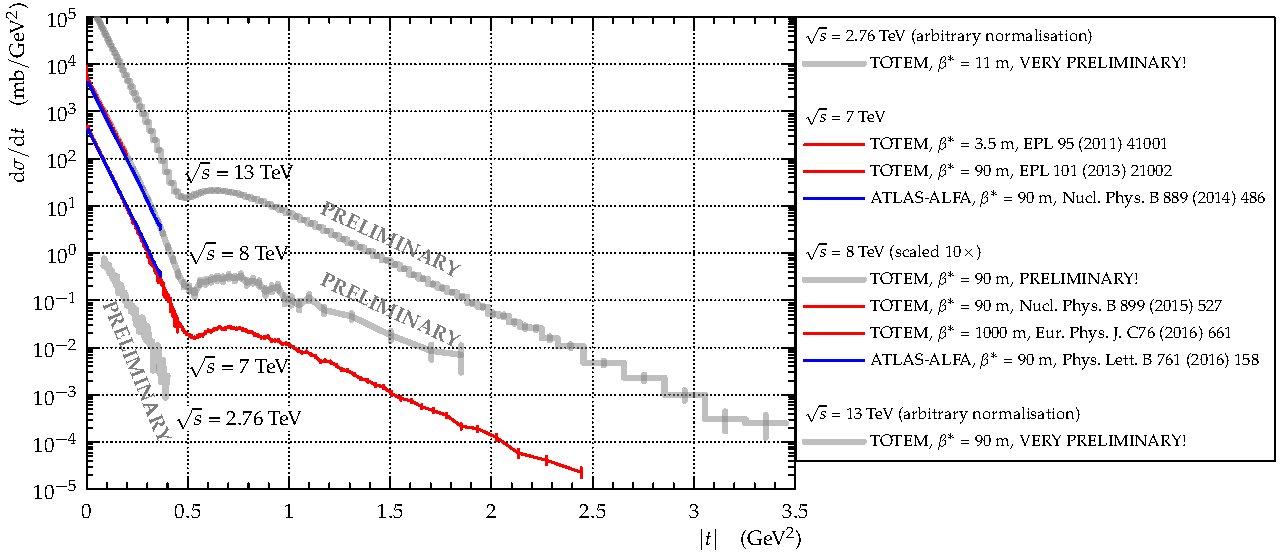
\includegraphics[height=6cm,clip]{fig/es_summary.pdf}
\vbox to0pt{\vss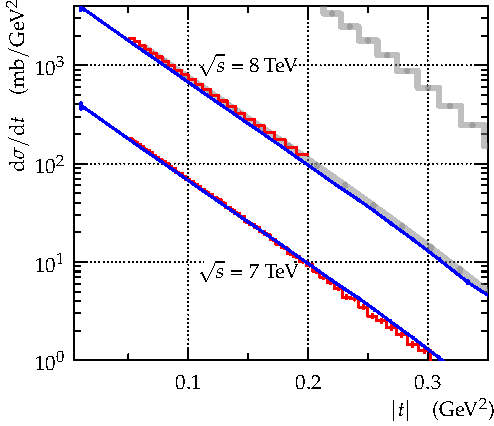
\includegraphics[height=3cm,clip]{fig/es_summary_detail_cone.pdf}\vskip3.3cm}
\vskip-7mm
\caption{A summary of elastic scattering differential cross-sections measured at LHC. The red and blue lines refer to measurements by TOTEM and ATLAS ALFA, respectively. The gray lines correspond to preliminary and yet unpublished data by TOTEM. Only statistical uncertainties are shown.}
\label{f:es summary}
\end{figure}

\section{Elastic scattering}
\label{s:es}

At the LHC there are two experiments instrumented to measure elastic scattering: ATLAS-ALFA and TOTEM. Their measurements are summarised in Figure~\ref{f:es summary}. Different regions of four-momentum transfer squared, $t$, probe different physics regimes of elastic scattering. At very low $|t|$, the interference between Coulomb and nuclear amplitudes (CNI) takes place. At larger values of $|t|$ up to $\approx 0.4\un{GeV^2}$, the differential cross-section presents almost exponential decrease sometimes called diffraction cone. This region is followed by a dip and a bump which are often explained by an interference of different amplitude components. At high values of $|t|$, where the cross-section exhibits a smooth and uniform decrease, one may expect a transition from non-perturbative to perturbative regime.

The inset of Figure~\ref{f:es summary} compares the measurements of ATLAS-ALFA and TOTEM which are in general in good agreement, especially regarding the slope. At $\sqrt s = 8\un{TeV}$, the measurement by ATLAS-ALFA is a little lower than the one by TOTEM which will be further discussed in Section~\ref{s:cs}

Figure~\ref{f:es summary} shows that the position of the dip moves to lower $|t|$ values with increasing energy: at $\sqrt s = 7\un{TeV}$ the dip occurs at $|t| \approx 0.53\un{GeV^2}$ while the preliminary data at $13\un{TeV}$ indicate it at about $|t| \approx 0.48\un{GeV^2}$.

The $\sqrt s = 13\un{TeV}$ TOTEM cross-section at high $|t|$ presents a uniform decrease. Although this measurement is preliminary, the yet to be applied corrections are unlikely to create any structures. This is contraction to predictions of many models where secondary dips or other oscillations can be observed. The TOTEM measurement, in turn, excludes all such models. In fact, it rules all models built on the optical analogy -- where multiple dips or oscillations are inevitable. On the other hand, the measurement may be favouring a hypothesis that large $|t|$ elastic scattering is dominated by a perturbative QCD amplitude, e.g.~triple gluon exchange proposed by Donnachie and Landshoff.

\begin{figure}[h]
\centering
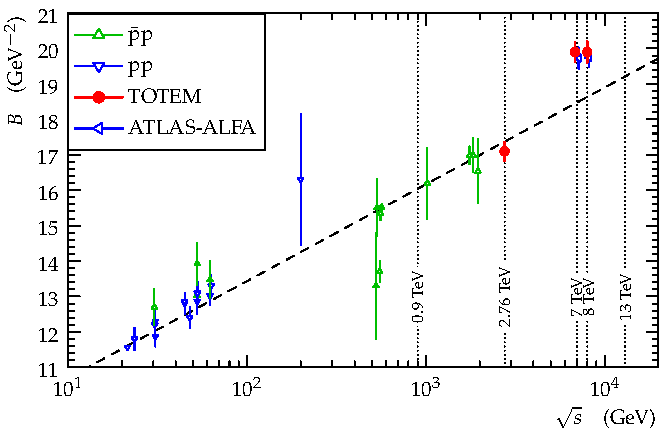
\includegraphics[height=6cm,clip]{fig/es_B_vs_s.pdf}
\vskip-4mm
\caption{Measurements for forward slope, $B$, as a function of energy. Data for $\rm pp$ and $\rm p\bar p$ are drawn in blue and green, respectively. TOTEM measurements are drawn in red. The dashed line represents a fit of pre-LHC data \cite{b-vs-s-data}.}
\label{f:es B}
\end{figure}


Figure~\ref{f:es B} summarises measurements of forward slope, $B$:
\begin{equation}
B = \left. {\d\over \d t} \log {\d\sigma\over \d t} \right|_{t = 0}\ .
\end{equation}
All measurements for $\sqrt s < 3\un{TeV}$ are compatible with a fit linear in $\log s$, see the dashed line. However, this trend is not respected by $\sqrt s = 7$ and $8\un{TeV}$ measurements by ATLAS-ALFA \cite{alfa-si-el-7tev,alfa-si-el-8tev} and TOTEM \cite{totem-si-el-7tev,totem-si-8tev} (well compatible with each other). This indicates an onset of new scattering regime between $\sqrt s = 2.76$ and $7\un{TeV}$. TODO: 13 TeV point


The diffraction cone presents differential cross-section with approximately exponential decrease. To visualise small deviations from this leading behaviour Figure~\ref{f:es non-exp} shows the relative difference of measured $\d\sigma/\d t$ from a reference exponential. All measurements, by ATLAS-ALFA \cite{alfa-si-el-7tev,alfa-si-el-8tev} and by TOTEM \cite{totem-si-el-7tev,totem-el-non-exp-8tev}, give a qualitatively similar picture at all available energies. For $|t| \lesssim 0.2\un{GeV^2}$ deviations with a ``U'' shape that were evaluated a more than $7\un{\sigma}$ significance in \cite{totem-el-non-exp-8tev}. For $|t| \gtrsim 0.2\un{GeV^2}$ the slope increases, thus the differential cross-section falls steeper towards the dip.

\begin{figure}[h]
\centering
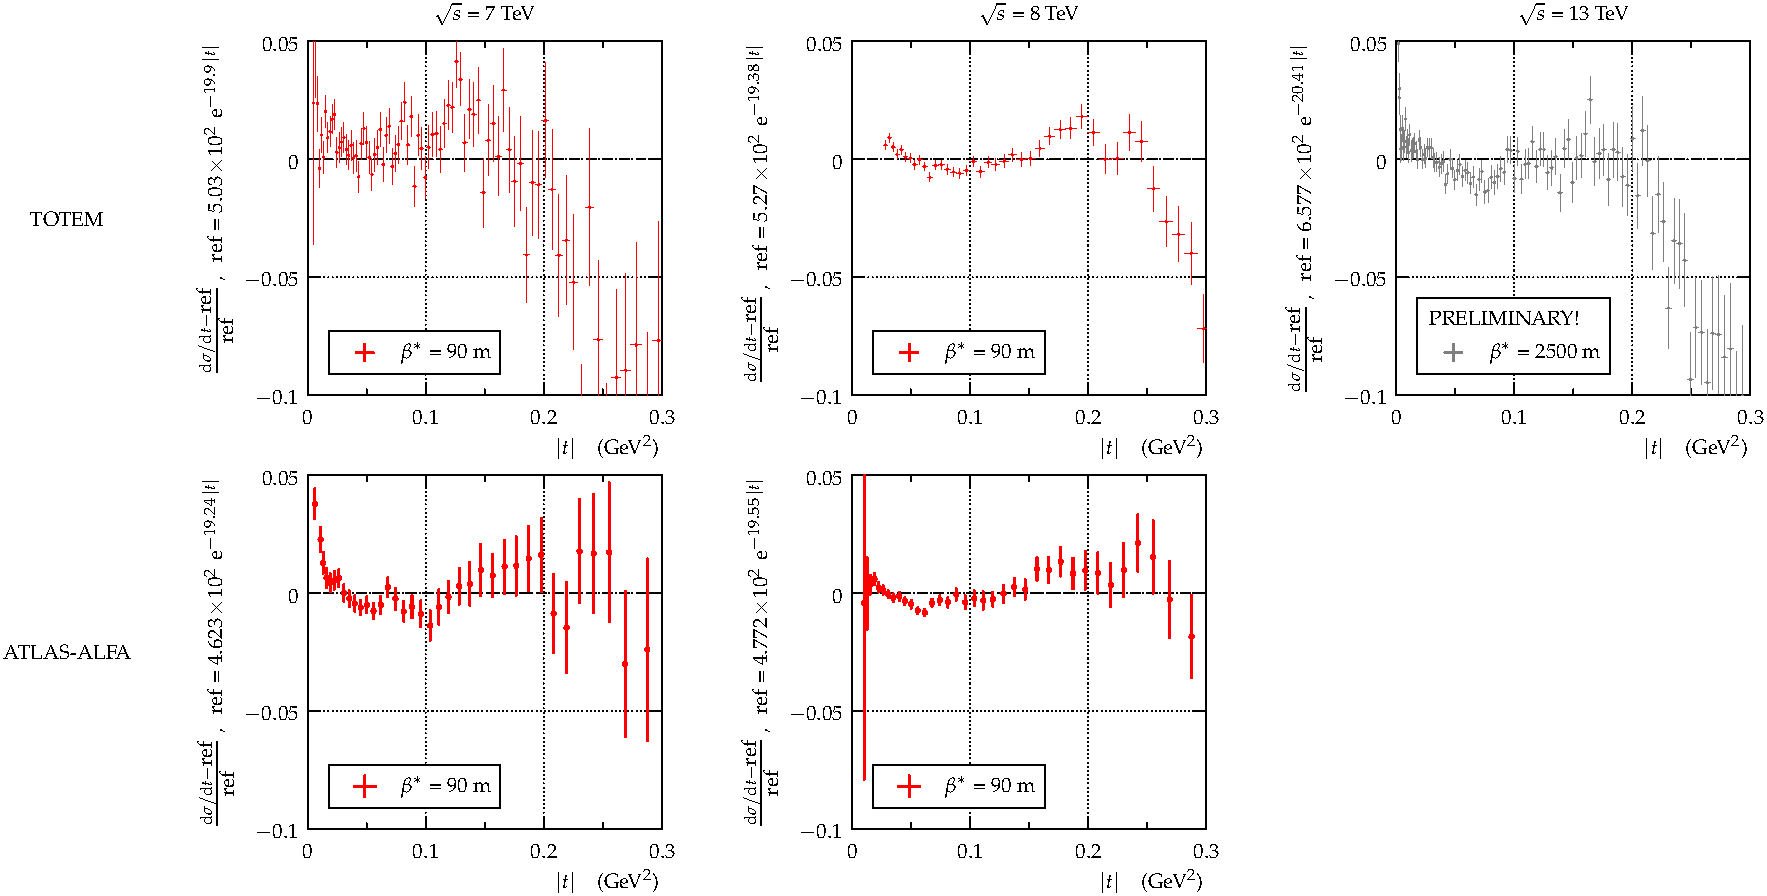
\includegraphics[height=6cm,clip]{fig/es_t_dist_rel_cmp.pdf}
\vskip-4mm
\caption{Details of the diffraction cone: relative deviation from a reference exponential. Top row: measurements by TOTEM, bottom row: measurements by ATLAS-ALFA.}
\label{f:es non-exp}
\end{figure}

\begin{figure}[h]
\centering
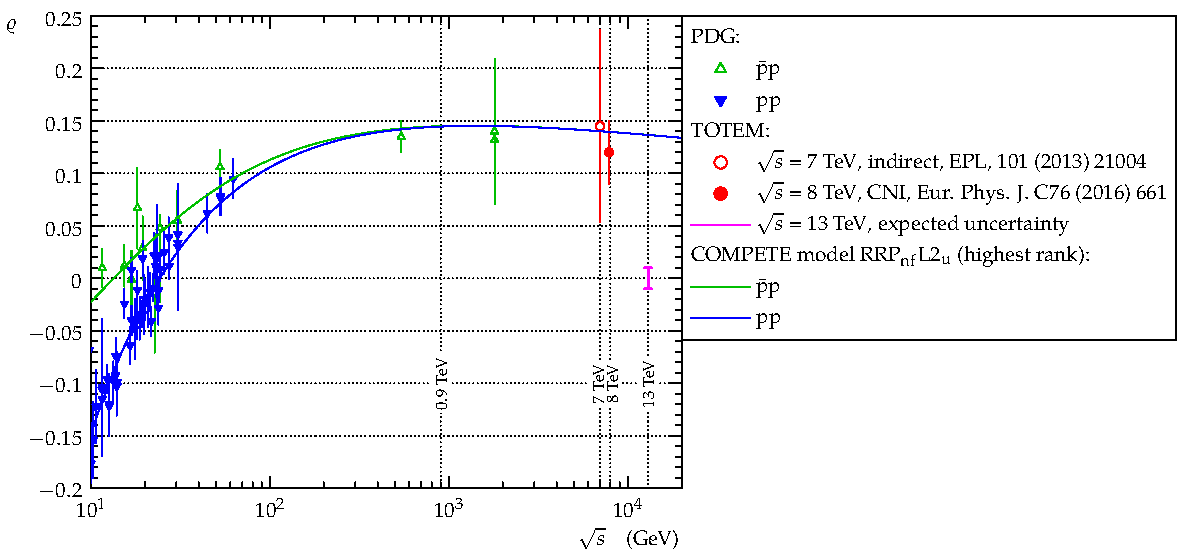
\includegraphics[height=6cm,clip]{fig/es_rho_vs_s.pdf}
\vskip-4mm
\caption{$\rho$ measurements plotted as a function of energy. The pre-LHC data are taken from collection \cite{pdg}. The solid lines represent pre-LHC fits by the COMPETE Collaboration \cite{compete}. Green and blue colours refer to $\rm p\bar p$ and $\rm pp$ scattering, respectively; TOTEM measurements are drawn in red.}
\label{f:es rho}
\end{figure}

Since the Coulomb scattering amplitude is calculable from QED, the CNI occurring at very low $|t|$ enables to determine the phase of the nuclear amplitude. This is typically quantified in terms of the $\rho$ parameter, the ratio of real to imaginary part of the nuclear scattering amplitude:
\begin{equation}
\rho = \left. {\Re {\cal A}^{\rm N} \over \Im {\cal A}^{\rm N}} \right|_{t = 0}\ .
\end{equation}
Figure~\ref{f:es rho} shows a compilation of $\rho$ measurements vs.~energy. ATLAS-ALFA has not published any result yet, but $\sqrt s = 8\un{TeV}$ measurement is in progress. TOTEM's measurement at this energy \cite{totem-8tev-1km} is little below but still compatible with the COMPETE extrapolations \cite{compete} due to the large uncertainty. At $\sqrt s = 13\un{TeV}$ TOTEM is aiming at $\rho$ uncertainty about $0.01$ which should be sufficient to probe the compatibility with the COMPETE models. This is interesting since deviations may indicate the existence of the Odderon (e.g.~\cite{nicolescu}), the even-under-crossing partner of the Pomeron. $\rho$ is particularly sensitive parameter since the real part of the Pomeron-exchange amplitude is expected small and therefore the contribution from the Odderon may be significant albeit it is generally dominated by the Pomeron. TODO: other channels?


%----------------------------------------------------------------------------------------------------
\section{Cross-sections}
\label{s:cs}

Figure~\ref{f:cs summary} shows a compilation of total, inelastic and elastic cross-sections. The pre-LHC data were taken from \cite{pdg} an additional cosmic-ray measurement is by the Auger Collaboration \cite{auger-57tev}. ATLAS-ALFA \cite{alfa-si-el-7tev,alfa-si-el-8tev} and TOTEM \cite{totem-si-tot-7tev,totem-si-8tev,totem-si-2.76tev} have contributed by several measurements of all three cross-sections. Additional inelastic cross-section measurements comprise results from ALICE \cite{alice-inel-sd-dd}, ATLAS \cite{atlas-inel-7tev,atlas-inel-13tev}, CMS \cite{cms-inel-7tev,cms-inel-13tev} and LHCb \cite{lhcb-inel-7tev}. $\sqrt s = 13\un{TeV}$ results from TOTEM are expected soon, ATLAS-ALFA has data at this energy to analyse, too. Furthermore, these two experiments aim at measurements at $\sqrt s = 0.9\un{TeV}$ possibly even at the end of 2017. This will constitute 5 sampling points and thus strong constraint for the energy dependence of the cross-section. The presently available data are compatible with $\log^2 s$ growth of all the cross-sections.

\begin{figure}[h]
\centering
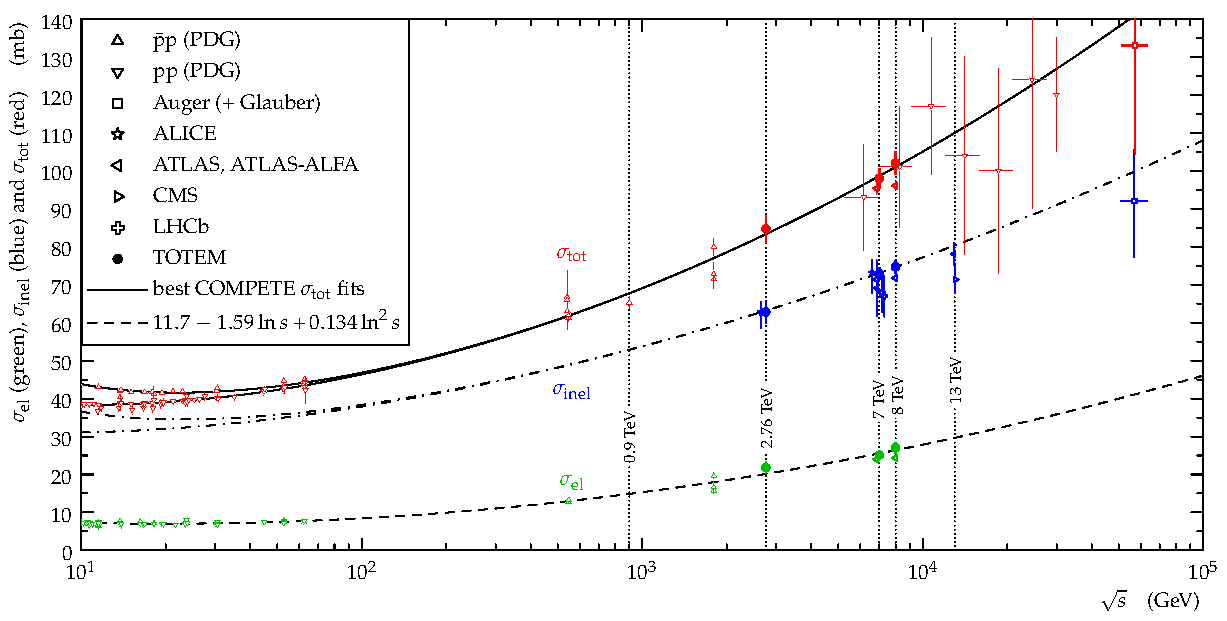
\includegraphics[height=6cm,clip]{fig/sigma_tot_el_inel_vs_s.pdf}
\vskip-4mm
\caption{Total (red), inelastic (blue) and elastic (green) cross-sections plotted as a function of energy. For references see text. The solid lines represent the pre-LHC fits by COMPETE \cite{compete}. The dashed line shows a $\sigma_{\rm el}$ fit by TOTEM, including its $7$ and $8\un{TeV}$ and PDG \cite{pdg} points. The dashed-dotted line corresponds to a difference between a $\sigma_{\rm tot}$ fit by COMPETE and the $\sigma_{\rm el}$ fit by TOTEM.}
\label{f:cs summary}
\end{figure}

It is interesting to compare the total cross-section measurements by ATLAS-ALFA and TOTEM. While the $\sqrt s = 7\un{TeV}$ points are fully compatible, there is about $2\un{\sigma}$ tension at $8\un{TeV}$. It can be traced down to the normalisation (thus to luminosity or inefficiency determination) of the differential cross-section, cf.~Figure~\ref{f:es summary}, inset. The two measurements therefore give quite different trends: while TOTEM points are compatible with the COMPETE fit, the ATLAS-ALFA points give extrapolation to $13\un{TeV}$ about $10\un{mb}$ lower. Consequently, the soon-available $13\un{TeV}$ results will shed light on this puzzle.

The comparison is even more complicated for the inelastic cross-section given the large variety of results. One can observe that while ALICE and TOTEM results are compatible with the dashed-dotted line, all others lie below. This can be understood by studying the systematic uncertainties related to each measurement. Those performed with central detectors only necessarily need to correct for events escaping the apparatus in the forward direction. This correction is sizeable and strongly model dependent. For example, the CMS analysis \cite{cms-inel-13tev} takes a ``democratic'' approach and uses a mean correction over a handful of Monte-Carlo predictions. In another example, the ATLAS analysis \cite{atlas-inel-13tev} first tunes and compares various models to data and for the final correction selects only those which describe the data well. This procedure tends to select models predicting larger corrections. In other words, unwise selection of Monte-Carlo predictions can lead to underestimation of the inelastic cross-section. This conclusion is supported also by $\sigma_{\rm inel}$ measurements by experiments including Roman Pots: ATLAS-ALFA and TOTEM can determine the inelastic cross-section by $\sigma_{\rm tot} - \sigma_{\rm el}$ and the results favour larger values. Finally, at $\sqrt s = 7\un{TeV}$ TOTEM determined the inelastic cross-section by 3 different methods \cite{totem-si-tot-7tev} and yielding consistent results compatible with the dash-dotted line.


%----------------------------------------------------------------------------------------------------
\section{Single diffraction}
\label{s:sd}

\begin{figure}[h]
\centering
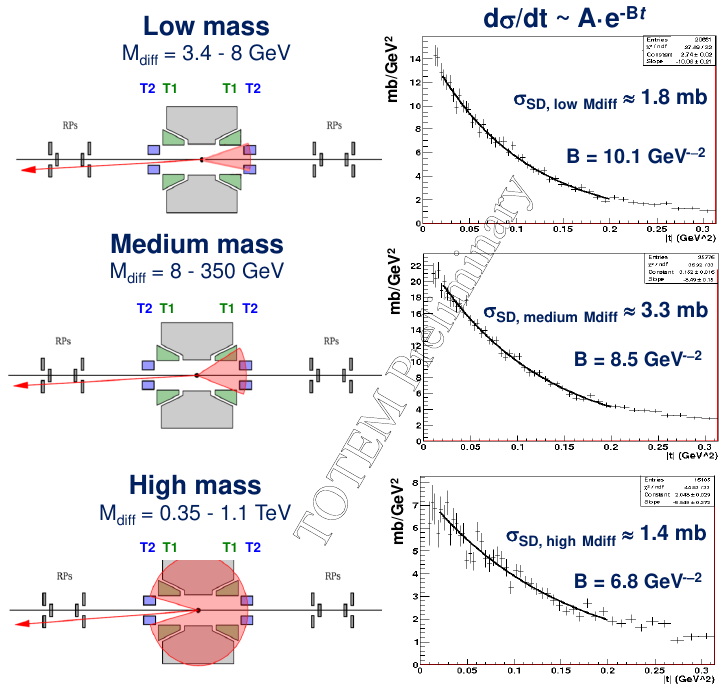
\includegraphics[height=6cm,clip]{fig/sd_7TeV.png}
\vskip-4mm
\caption{Illustration of TOTEM single diffraction measurement, adapted from slides by H.~Saarikko.}
\label{f:sd TOTEM}
\end{figure}

ALICE has published \cite{alice-inel-sd-dd} a single-diffraction measurement based on counting events with single-sided topology. The surviving protons were not tagged in this analysis and only integrated cross-sections are presented, see Figure~\ref{f:sd cs summary}.

CMS has published \cite{cms-diff-7tev} a measurement based on counting events with rapidity gaps on one side of the detector. Also in this analysis the forward protons were not identified. The cross-section was presented as a function of $\xi$, the fractional momentum loss: showing a gentle decrease of the cross-section with $\xi$, where none of the studied Monte-Carlo generators was able describe all the features.

TOTEM has preliminary (not yet published) results from an analysis at $\sqrt s = 7\un{TeV}$ where the surviving protons are tagged. As illustrated in Figure~\ref{f:sd TOTEM}, the analysis is performed in 3 diffractive mass (or $\xi$) bins. They are defined by the acceptance of TOTEM subdetectors and the relation between the rapidity gap, $\Delta y$ and $\xi$: $\Delta y \approx -\log\xi$. For each $\xi$ bin, the results presented as a function of the proton four-momentum transfer squared, $t$. The distributions are compatible with exponentials with the slope, $B$, decreasing with increasing $\xi$. Summing the preliminary cross-sections values yields $(6.5\pm 1.3)\un{mb}$. This can be complemented with a cross-section of $(2.6\pm 2.2)\un{mb}$ which corresponds to events with particles more forward than the T2 acceptance \cite{totem-si-inel-7tev}. As this cross-section is expected to be dominated by single diffraction, one can estimate $\sigma_{\rm SD} = (9.1 \pm 2.9)\un{mb}$. This value corresponds to cutoff $\xi \lesssim 0.022$ and is represented by the green point in Figure~\ref{f:sd cs summary}.

There is also an ongoing combined CMS + TOTEM analysis at $\sqrt s = 8\un{TeV}$ which combines the benefits of a central detector and forward-proton taggers. This analysis aims at event classification as non-diffractive, single-diffractive and double-diffractive.

\begin{figure}[h]
\centering
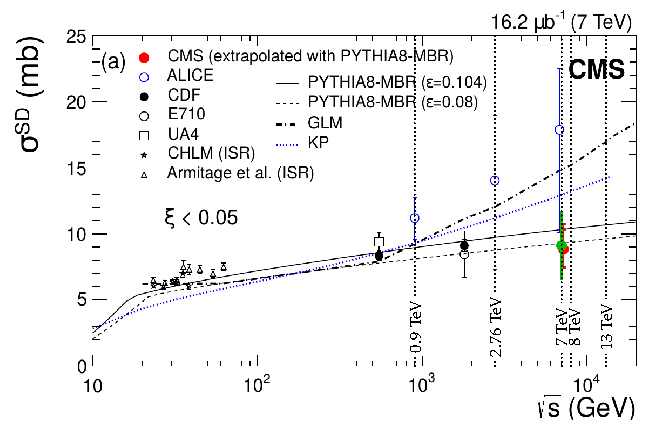
\includegraphics[height=6cm,clip]{fig/si_sd_vs_s.pdf}
\vskip-4mm
\caption{Single-diffractive cross-section as a function of energy. Plot adapted from \cite{cms-diff-7tev}. The ALICE data are from \cite{alice-inel-sd-dd}. The green point corresponds to a compilation of TOTEM data, see text.
}
\label{f:sd cs summary}
\end{figure}

ATLAS published a study of events with rapidity gaps \cite{atlas-rap-gap-7tev} at $\sqrt s = 7\un{TeV}$ where, however, no attempt was made to disentangle non-diffractive, single-diffractive and double-diffractive components.


%----------------------------------------------------------------------------------------------------
\section{Double diffraction}
\label{s:dd}

ALICE has published \cite{alice-inel-sd-dd} a double-diffraction measurement based on counting events with central rapidity gap $\Delta\eta > 3$. Only integrated cross-sections are presented, see Figure~\ref{f:dd cs summary}.

CMS has published \cite{cms-diff-7tev} a similar measurement, also counting events with central rapidity gap $\Delta\eta > 3$. The results are presented as a function of the rapidity gap, featuring decreasing cross-section with increasing gap size.

TOTEM made a measurement at $\sqrt s = 7\un{TeV}$ \cite{totem-dd-7tev} however constrained to a narrow fiducial region where background could be controlled and subtracted. Consequently, no attempt to extrapolate to the full phase space was made.

As mentioned in Section~\ref{s:sd}, the combined CMS + TOTEM analysis is expected to provide double-diffraction cross-section at $\sqrt s = 8\un{TeV}$.

\begin{figure}[h]
\centering
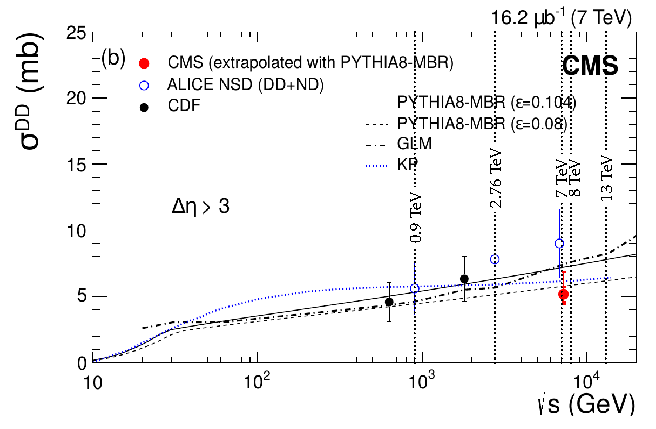
\includegraphics[height=6cm,clip]{fig/si_dd_vs_s.pdf}
\vskip-4mm
\caption{Double-diffractive cross-section as a function of energy. Plot adapted from \cite{cms-diff-7tev}. The ALICE data are from \cite{alice-inel-sd-dd}.}
\label{f:dd cs summary}
\end{figure}

%----------------------------------------------------------------------------------------------------

% TODO: order

\begin{thebibliography}{}
% TODO: remove
% Format for books
%\bibitem{RefB}
%	Book Author, \textit{Book title} (Publisher, place, year) page numbers

\bibitem{alice}
	ALICE Collaboration, J.~Instrum.~\textbf{3}, S08002 (2008)

\bibitem{atlas}
	ATLAS Collaboration, J.~Instrum.~\textbf{3}, S08003 (2008)

\bibitem{cms}
	CMS Collaboration, J.~Instrum.~\textbf{3}, S08004 (2008)

\bibitem{lhcb}
	CMS Collaboration, J.~Instrum.~\textbf{3}, S08005 (2008)

\bibitem{totem}
	G. Anelli et al. (TOTEM Collaboration), J.~Instrum.~\textbf{3}, S08007 (2008)

\bibitem{pdg}
	K.~Nakamura et al. (Particle Data Group), J.~Phys.~G \textbf{37}, 075021 (2010)

\bibitem{compete}
	J.~R.~Cudell et al.~(COMPETE Collaboration), Phys.~Rev.~Lett.~\textbf{89}, 201801 (2002)

\bibitem{alfa-si-el-7tev}
	ATLAS Collaboration, Nucl.~Phys.~B \textbf{889}, 486--548 (2014)

\bibitem{alfa-si-el-8tev}
	ATLAS Collaboration, Phys.~Lett.~B \textbf{761}, 158--178 (2016)

\bibitem{totem-si-el-7tev}
	TOTEM Collaboration, Europhys.~Lett.~\textbf{101}, 21002 (2013)

\bibitem{totem-si-inel-7tev}
	TOTEM Collaboration, Europhys.~Lett.~\textbf{101}, 21003 (2013)

\bibitem{totem-si-8tev}
	TOTEM Collaboration, Phys.~Rev.~Lett.~\textbf{111}, 012001 (2013)

\bibitem{totem-si-2.76tev}
	TOTEM Collaboration, publication in preparation

\bibitem{totem-si-tot-7tev}
	TOTEM Collaboration, Europhys.~Lett.~\textbf{101}, 21004 (2013)

\bibitem{totem-el-non-exp-8tev}
	TOTEM Collaboration, Nucl.~Phys.~B \textbf{899}, 527--546 (2015)

\bibitem{totem-8tev-1km}
	TOTEM Collaboration, Eur.~Phys.~J.~C \textbf{76}, 661 (2016)

\bibitem{b-vs-s-data}
	\Name{ISR (CR Collaboration)}, \REVIEW{Phys.~Lett.}{B62}{1976}{460}; 
	\Name{ISR (ACHGT Collaboration)}, \REVIEW{Phys.~Lett.}{B39}{1972}{663}; 
	\Name{ISR (R-211)}, \REVIEW{Nucl.~Phys.}{B262}{1985}{689}; 
	\Name{ISR (R-210)}, \REVIEW{Phys.~Lett.}{B115}{1982}{495}; 
	\Name{UA1}, \REVIEW{Phys.~Lett.}{B147}{1984}{385}; 
	\Name{UA4}, \REVIEW{Phys.~Lett.}{B127}{1983}{472} and \REVIEW{Phys. Lett.}{B198}{1987}{583}; 
	\Name{UA4/2}, \REVIEW{Phys.~Lett.}{B316}{1993}{448}; 
	\Name{CDF}, \REVIEW{Phys.~Rev.}{D50}{1994}{5518}; 
	\Name{E710}, \REVIEW{Phys.~Rev.~Lett.}{68}{1992}{2433} and \REVIEW{Nuovo Cimento}{A106}{1992}{123}; 
	\Name{D0}, D0 Note 6056-CONF; 
	\Name{pp2pp}, \REVIEW{Phys.~Lett.}{B579}{2004}{245}

\bibitem{nicolescu}
	TODO

\bibitem{auger-57tev}
	P. Abreu et al. (Pierre Auger Collaboration), Phys.~Rev.~Lett. \textbf{109}, 062002 (2012)

\bibitem{alice-inel-sd-dd}
	ALICE Collaboration, Eur.~Phys.~J.~\textbf{C73}, 2456 (2013)

\bibitem{atlas-inel-7tev}
	ATLAS Collaboration, Nature Commun.~\textbf{2}, 463 (2011)

\bibitem{atlas-inel-13tev}
	ATLAS Collaboration, Phys.~Rev.~Lett.~\textbf{117}, 182002 (2016)

\bibitem{cms-inel-7tev}
	CMS Collaboration, CMS-PAS-FWD-11-001, https://cds.cern.ch/record/1373466

\bibitem{cms-inel-13tev}
	CMS Collaboration, CMS-PAS-FSQ-15-005, https://cds.cern.ch/record/2145896

\bibitem{lhcb-inel-7tev}
	LHCb collaboration, J. High Energ. Phys. \textbf{02}, 129 (2015)

\bibitem{cms-diff-7tev}
	CMS Collaboration, CMS-PAS-FSQ-12-005; arXiv:1503.08689

\bibitem{totem-dd-7tev}
	TOTEM Collaboration, Phys.~Rev.~Lett.~\textbf{111}, 262001 (2013)


\end{thebibliography}

\end{document}
